\documentclass{ctexart}
\usepackage{graphicx}
\usepackage{hyperref}

\begin{document}

\title{SatuFS 最终设计报告}
\author{马凯,李文睿,刘时,金孜达}
\date{}
\maketitle

\section{项目介绍}
\label{sec:intro}

本组的项目为 SatuFS,是一个面向物联网的文件系统。其主要功能为将不同类型
的网络连接持久化存储在文件中,从而在网络数据高效传输的同时,可以做到近
乎实时的缓冲和备份,并且对用户提供一个一致且易用的接口。

\section{立项依据}
\label{sec:background}

现在,物联网技术正在广泛而深刻地改变着我们的生活。但与物联网技术的汹汹
来势不同的是,我们发现开发可靠的物联网应用门槛较高,这意味着要么忍受低
质量的软件,要么忍受过长的开发周期。

鉴于网络在物联网应用中的重要地位,我们提出了 SatuFS,即如何在网络高效和
可靠之间达成平衡,甚至是两全其美。我们注意到物联网应用所在网络常常处于
不稳定状态,于是开始思考“可否在断网时自动缓冲数据,上线时再将这些数据
发出去?”这就是我们项目的动机。

\section{设计与实现}
\label{sec:arch}

本节概述了我们项目目前的设计与实现。

\subsection{总体设计}
\label{sec:overall}

从第 \ref{sec:background} 节可以看出,SatuFS 项目并非独立的文件系统,要
使之可以正常工作,必须有配套的通讯协议和服务端。由于目前大部分物联网系
统都有一个中心节点,出于实用性和简单性考虑,我们简单地将我们的整体系统
设计为星形结构(如图 \ref{fig:network})。

\begin{figure}
  \centering
  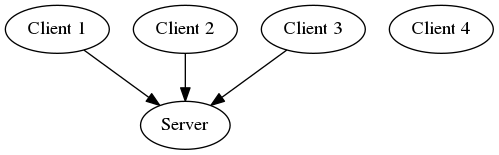
\includegraphics[scale=0.4]{design-net-topo.png}
  \caption{网络结构}
  \label{fig:network}
\end{figure}

我们并未实现所有设计。已经有设计且我们认为有望实现的但尚未实现的均使用
楷体。

\subsection{可移植性设计}
\label{sec:port}

出于开发环境友好程度考虑,我们首选 RIOT 为开发平台,但考虑到 FreeRTOS
在业界的统治地位,我们也不能完全忽视之。因此,我们借鉴了 RIOT 的 pkg 机
制,采用了分层式可移植的设计(如图 \ref{fig:port})。

\begin{figure}
  \centering
  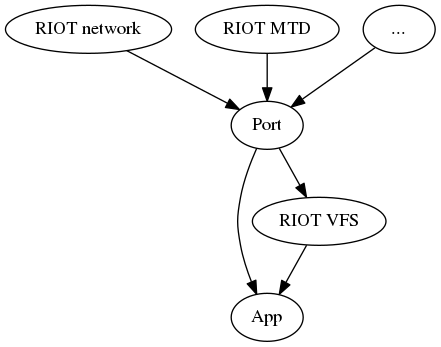
\includegraphics[scale=0.4]{portability1.png}
  \caption{可移植设计示意图}
  \label{fig:port}
\end{figure}

其中,Port 是胶合层,在移植 SatuFS 时仅需重写 Port 即可。而 Port 用来做
这些事:

\begin{enumerate}
\item 提供与系统相关的接口:闪存设备的读、烧写、擦除,网络的连接、数据
  发送、数据接收,创建任务等。
\item 面对最终用户提供配置接口:最大网络连接数,文件系统相关参数设置
  等。
\end{enumerate}

目前我们仅实现了 RIOT 的 port。

\subsection{网络操作与协议设计}
\label{sec:network}

当前 SatuFS 仅支持 UDP 协议。UDP 与 TCP 的一大区别是,UDP 是不可靠的面
向数据报文的协议。如何检测网络连接断开是一大困难。为此,我们简单地使用
了服务器发回确认数据的做法。

当服务端接受到来自客户端的数据时,服务端将自动发回 2 字节的确认消息(目
前这个消息并没有实质性意义)。客户端阻塞地尝试读取这个确认,如果在指定
超时时间后还没有读到,或读到的消息不完整,则认为网络连接已断开。

由于 RIOT 本身对 TCP 支持弱于 UDP,因此我们没有实现 TCP 版本。事实上,
由于 SatuFS 的层次设计,切换到 TCP 或 UDP 并不困难。

\subsection{数据管道设计}
\label{sec:pipe}

在 RIOT 中,数据管道意味着写入该文件的数据将如同被管道送走一样,送向远
程服务器。我们设计了流数据管道和消息数据管道。

在可行性报告中,我们提出了一种设计,即实现全新的文件类型,与目录、常规
文件等同。但在实现时,我们发现在这种设计下,网络连接的控制信息没有很好
的途径传递给文件系统(即使考虑 \verb|fcntl|),且 VFS 通常会进行一些重
解释的操作,这导致我们无法对 flags 进行自定义,因此我们提出了{\heiti 工
  作模式}的概念来绕过这些限制。

工作模式仅对常规文件来讲。有三种工作模式:

\begin{enumerate}
\item 常规工作模式(regular):该模式为默认设置;在这种模式下,对文件的
  操作就是对存储媒介上物理文件的操作。
\item 流数据工作模式(stream,\ref{sec:stream}):对文件的写操作将被发
  送到远程服务器;{\kaishu 一个可读的流数据文件将自动缓冲服务器发来的数
    据,在请求读时立即返回已有数据};网络断开时自动进行缓冲。
\item {\kaishu 消息工作模式(message,\ref{sec:message})}
\end{enumerate}

使用 \verb|fcntl| 在不同的模式间切换。


\subsubsection{流数据管道设计}
\label{sec:stream}

在首次切换到流数据管道前,需在常规模式下写入如下格式的控制信息:

\begin{verbatim}
typedef struct {
    char magic[4];
    uint16_t port;
    char addr[256];
    uint32_t buffer_size;
    uint32_t head;
    uint32_t tail;
} satufs_stream_info_t;
\end{verbatim}

其中 \verb|magic| 为字符串 ``satu'',\verb|port| 为远程服务器端口
号,\verb|addr| 为远程服务器的 IPv6 地址(字符串格式\footnote{\kaishu
  如果并非 IPv6,可以回退到 DNS 查询。}),\verb|buffer_size| 为所用缓冲
区的大小,\verb|head| 和 \verb|tail| 是文件系统用于持久化存储控制信息所
用,用户不需关心。

由于将控制信息与函数调用分离,我们可以轻松地在未来扩展这些信息。

这些控制信息和缓冲数据将被持久化存储在文件中,即文件系统卸载并重新挂载
后,仍可读取并利用这些信息。

在确保流数据管道文件正确初始化过后,可以使用 \verb|fcntl| 切换工作模式
到流模式:

\begin{verbatim}
fcntl(fd, SATU_SETMODE, SATU_MODE_STR)
\end{verbatim}

在 \verb|fcntl| 中,SatuFS 将进行以下工作:

\begin{enumerate}
\item 连接到远程服务器,并将连接保存在内存中,如果连接失败,就认为网络
  一开始就是断线的。这一步将永远不会失败。
\item 预先分配缓冲区空间,如果失败,说明磁盘空间不足,返回错误。
\item 切换工作模式。
\end{enumerate}

若 \verb|fcntl| 返回成功,就说明流数据管道可以正常工作了。

当发生 \verb|write| 时,SatuFS 将进行以下工作:

\begin{enumerate}
\item 尝试清空缓冲区(尽量保证流数据按生成顺序发出),如果不能全部发送,
  转 \ref{stash}。
\item 尝试发送本次的所有数据,如果不能全部发送,转 \ref{stash};如果成
  功地发送出了全部数据,返回成功。
\item \label{stash} 将未能成功发出的数据保存在缓冲区内。
\end{enumerate}

可见 SatuFS 对流数据文件的写操作将永远不会失败。网络数据发送见
节 \ref{sec:network}。当尝试将数据保存在缓冲区内时,如果缓冲区已满,就
覆盖掉最早进入缓冲区的数据(FIFO 替换策略)。

对于读操作,我们仅有设计,并未实现。

{
  \kaishu

  在支持异步通知的系统上,在数据到达时直接插入缓冲区,读取时立即返回数
  据。

  但很多嵌入式系统(如 RIOT)并不支持异步通知,在这些不支持异步通知的系
  统上,可能需要用户程序作出适应性修改。

  \begin{itemize}
  \item 创建读者线程,该线程阻塞在 \verb|recv| 操作上,拥有较低优先级;
    如果数据到达,则插入缓冲区。
  \item 用户线程时不时地进行休眠,给予读者线程执行机会。
  \end{itemize}

  由于这两种模式有强烈的冲突,限于嵌入式开发经验,我们很难作出决定。如
  果两种做法都支持,那么 SatuFS 将失去“毋须修改用户代码”的可移植性。
}

\subsubsection{消息数据管道设计}
\label{sec:message}

{
  \kaishu

  消息数据管道与流数据管道的不同在于,消息数据管道是以一个结构化的消息
  为原子,而非字节级别的原子操作。

  当消息数据发出时,首先将消息缓存,再尝试发出。读取消息与读流数据类
  似。

  由于消息的结构化、(一般)不定长特征,消息头部需附有 SatuFS 的一些控
  制信息。

}

\subsubsection{服务端设计}
\label{sec:server}

SatuFS 的服务端的主要设计目标是:

\begin{itemize}
\item 可以储存流数据{\kaishu 和消息数据}。
\item 可以分析数据并作出反应。
\item 提供扩展接口并允许用户进行拓展和二次开发。
\end{itemize}

这些目标也基本达成了。目前,服务端是一个使用 Python 编写的简单的测试用
服务器。

\section{成果}
\label{sec:result}

一定程度上,我们取得了预期成果,但并未完成全部目标。我们目前取得的成果
为:

\begin{itemize}
\item 可移植性:仅需实现若干接口,即可简单地将 SatuFS 移植到不同文件系
  统上,而用户代码和 SatuFS 本体代码无需任何改动。
\item 高可用性:按目前的实现,管道文件的写操作将永远不会失败,在一定限
  度内,数据将不会丢失。
\item 可靠性:未发出的数据将被合理处理,而不会因为网络原因丢失。
\end{itemize}

此外,我们编写了一个简单的测试程序和测试服务器,分别在 \verb|/example|
和 \verb|/server| 目录下。测试仅需在 \verb|/example| 目录下执
行 \verb|make all term| 即可。

SatuFS 项目的本质是将网络连接的文件化,这与 Plan 9 有一定相似之处,但与
之不同的是我们并未提供一个单独的控制文件,也将网络连接的控制信息持久化
地储存在文件中。我们认为本项目在文件概念抽象的发展上仍有一定前景,即将
网络连接和数据文件均视为广义的文件。此外,我们认为工作模式的概念也对其
他文件系统有启发和借鉴意义,它可以在减少文件系统内部冗余、提供一致接口
的情况下丰富文件系统的功能。

\section{未来改进}
\label{sec:future}

截至目前,本项目仍有较大的改进空间:

\begin{itemize}
\item 实现项目的其他设计:
\item 进一步提高可移植性:文件系统有些数据在持久化存储的时候没有统一字
  节序,需要修正。
\item 提高项目的可靠性:项目中有一些断言未经检验,也有一些因为缺失功能
  造成的可靠性降低,这部分可以进行改进。
\end{itemize}

\section{回顾与总结}
\label{sec:conclusion}

本项目并非本组提出的第一个项目,而是脱胎于一开始的一个分布式文件系统构
想,在遇到物联网这一题目后才被完整提出。

在确立题目后,我们通过阅读网络上的资料,特别是 FreeRTOS 的文档,调研学
习了物联网的概念、实时操作系统的基本概念和实现、存储技术设备、文件系统
的设计、网络服务器开发等广泛的内容。

与预期完成的目标相比,我们仅实现了一部分。这与我组的沟通不畅和效率低下
有关。我们在项目早期每周进行一次会议,但每次会议常常陷入细节的争论,且
没有明确主题,这导致会议效率过低。后来主要通过在线渠道联络,但经常无法
取得联系,导致项目长期内没有进展。此外,每个人的职责没有明确,组员对项
目本身兴趣不大,这些也是重要因素。

这次的合作经历成效较低,没有给每个人带来足够的发展和进步,也没有完成既
定目标。这对我们每个人都是一个教训,操作系统课程已经结束,现在已经没有
回头之路。这次的失败经历只能警醒我们在未来继续加油了!

\end{document}
